\documentclass[twoside]{book}

% Packages required by doxygen
\usepackage{fixltx2e}
\usepackage{calc}
\usepackage{doxygen}
\usepackage{graphicx}
\usepackage[utf8]{inputenc}
\usepackage{makeidx}
\usepackage{multicol}
\usepackage{multirow}
\PassOptionsToPackage{warn}{textcomp}
\usepackage{textcomp}
\usepackage[nointegrals]{wasysym}
\usepackage[table]{xcolor}

% Font selection
\usepackage[T1]{fontenc}
\usepackage{mathptmx}
\usepackage[scaled=.90]{helvet}
\usepackage{courier}
\usepackage{amssymb}
\usepackage{sectsty}
\renewcommand{\familydefault}{\sfdefault}
\allsectionsfont{%
  \fontseries{bc}\selectfont%
  \color{darkgray}%
}
\renewcommand{\DoxyLabelFont}{%
  \fontseries{bc}\selectfont%
  \color{darkgray}%
}
\newcommand{\+}{\discretionary{\mbox{\scriptsize$\hookleftarrow$}}{}{}}

% Page & text layout
\usepackage{geometry}
\geometry{%
  a4paper,%
  top=2.5cm,%
  bottom=2.5cm,%
  left=2.5cm,%
  right=2.5cm%
}
\tolerance=750
\hfuzz=15pt
\hbadness=750
\setlength{\emergencystretch}{15pt}
\setlength{\parindent}{0cm}
\setlength{\parskip}{0.2cm}
\makeatletter
\renewcommand{\paragraph}{%
  \@startsection{paragraph}{4}{0ex}{-1.0ex}{1.0ex}{%
    \normalfont\normalsize\bfseries\SS@parafont%
  }%
}
\renewcommand{\subparagraph}{%
  \@startsection{subparagraph}{5}{0ex}{-1.0ex}{1.0ex}{%
    \normalfont\normalsize\bfseries\SS@subparafont%
  }%
}
\makeatother

% Headers & footers
\usepackage{fancyhdr}
\pagestyle{fancyplain}
\fancyhead[LE]{\fancyplain{}{\bfseries\thepage}}
\fancyhead[CE]{\fancyplain{}{}}
\fancyhead[RE]{\fancyplain{}{\bfseries\leftmark}}
\fancyhead[LO]{\fancyplain{}{\bfseries\rightmark}}
\fancyhead[CO]{\fancyplain{}{}}
\fancyhead[RO]{\fancyplain{}{\bfseries\thepage}}
\fancyfoot[LE]{\fancyplain{}{}}
\fancyfoot[CE]{\fancyplain{}{}}
\fancyfoot[RE]{\fancyplain{}{\bfseries\scriptsize Generated on Fri Nov 14 2014 19\+:35\+:16 for Inter House Quiz Competition System by Doxygen }}
\fancyfoot[LO]{\fancyplain{}{\bfseries\scriptsize Generated on Fri Nov 14 2014 19\+:35\+:16 for Inter House Quiz Competition System by Doxygen }}
\fancyfoot[CO]{\fancyplain{}{}}
\fancyfoot[RO]{\fancyplain{}{}}
\renewcommand{\footrulewidth}{0.4pt}
\renewcommand{\chaptermark}[1]{%
  \markboth{#1}{}%
}
\renewcommand{\sectionmark}[1]{%
  \markright{\thesection\ #1}%
}

% Indices & bibliography
\usepackage{natbib}
\usepackage[titles]{tocloft}
\setcounter{tocdepth}{3}
\setcounter{secnumdepth}{5}
\makeindex

% Hyperlinks (required, but should be loaded last)
\usepackage{ifpdf}
\ifpdf
  \usepackage[pdftex,pagebackref=true]{hyperref}
\else
  \usepackage[ps2pdf,pagebackref=true]{hyperref}
\fi
\hypersetup{%
  colorlinks=true,%
  linkcolor=blue,%
  citecolor=blue,%
  unicode%
}

% Custom commands
\newcommand{\clearemptydoublepage}{%
  \newpage{\pagestyle{empty}\cleardoublepage}%
}


%===== C O N T E N T S =====

\begin{document}

% Titlepage & ToC
\hypersetup{pageanchor=false,
             bookmarks=true,
             bookmarksnumbered=true,
             pdfencoding=unicode
            }
\pagenumbering{roman}
\begin{titlepage}
\vspace*{7cm}
\begin{center}%
{\Large Inter House Quiz Competition System \\[1ex]\large v1.\+0 }\\
\vspace*{1cm}
{\large Generated by Doxygen 1.8.8}\\
\vspace*{0.5cm}
{\small Fri Nov 14 2014 19:35:16}\\
\end{center}
\end{titlepage}
\clearemptydoublepage
\tableofcontents
\clearemptydoublepage
\pagenumbering{arabic}
\hypersetup{pageanchor=true}

%--- Begin generated contents ---
\chapter{Main Page}
\label{index}\hypertarget{index}{}\subsection*{Introduction}

This is the repository of Inter-\/house quiz competition system, originally developed for S\+K\+H Tang Shiu Kin Secondary School of Hong Kong by One\+One Star, Steven Chien, Charlie Shum and Alfred Tai. This R\+E\+A\+D\+M\+E would normally document whatever steps are necessary to get your application up and running.

\subsection*{Summary}

The system consists of four major components\+: the database, event driven web server, main quiz server and buzzing system.

\subsubsection*{Database}

S\+Q\+Lite is used for storage of questions and answers as well of scores obtained by participants.

\subsubsection*{Event-\/driven web server}

A python web server utilizing Twisted library is used to receive instruction from quiz server and push changes to client web browsers.

\subsubsection*{Quiz Server}

A single threaded, non-\/blocking server written in C is used to act as a centralized server to store states of the game and communicate with various sub systems. The server uses libevent for buffering and create non-\/blocking sockets, S\+Q\+Lite A\+P\+I for database communication.

\subsubsection*{User Interface App}

The App acts as the control panel for the game maker where he can\+:


\begin{DoxyItemize}
\item Assign scores to participants
\item Display questions
\item Display answers
\item Control the display of elements in web page
\item Initiate and stop buzzing

All by communicating directly with the quiz server. The application is written in Java and undergoing transition to become an Android App.
\end{DoxyItemize}

\subsubsection*{Buzzing System}

A buzzing system consists of physical buttons where the first player who pressed the button gets to answer the question. The system consists of a Arduino Uno with program written in C++ and Raspberry Pi where communication between quiz server and Arduino is being bridged by program written in Python. The buzzing system is being controlled by the User Interface App.

\subsection*{Version}

The system was initially released in fall 2013.

\subsection*{Setup}

Sub system of the system can be started and restarted individually. In case of the buzzing system, it is started alone and connected to the network where the quiz server is hosted.

\subsubsection*{Start up}


\begin{DoxyEnumerate}
\item Web Server
\end{DoxyEnumerate}

Enter the directory where the server exists. Start the server by issuing the command as root\+: python server.\+py. Make sure that port 80 is not occupied by other program(i.\+e. Apache).


\begin{DoxyEnumerate}
\item Buzzing system
\end{DoxyEnumerate}

First make sure the Arduino is properly connected to the Raspbery Pi and powered. Execute the python program on Raspberry Pi and it will start waiting for connection.


\begin{DoxyEnumerate}
\item Quiz Server
\end{DoxyEnumerate}

The Quiz Server should be started when all sub systems are running. Execute by ./quiz\+\_\+server \mbox{[}I\+P addr of web server\mbox{]} \mbox{[}I\+P addr of the buzzing system(raspberry pi)\mbox{]}. The quiz server communicates with the web server through port 8889 and buzzing server through 8888.


\begin{DoxyEnumerate}
\item User Control Panel
\end{DoxyEnumerate}

The control panel is starting by inputting the I\+P address of quiz server. The default port of communication is 9000.

When all the above are started properly, the system should be ready to go.

\subsection*{Configuration}

The system occupies port 80, 8888, 8889 and 9000. Please make sure they are all open and not occupied on both sides.

\subsection*{Dependencies}

The system uses the below libraries\+:


\begin{DoxyItemize}
\item libevent
\item S\+Q\+Lite
\item Ncurses
\item G\+Lib
\item Various Linux system libraries
\end{DoxyItemize}

It is assumed the system will be used on Linux/\+U\+N\+I\+X platform.

\subsection*{Database setup}

The S\+Q\+Lite database for scores will be initialized if not exist or else the existing database will be used and scores will be automatically loaded upon initialization.

The S\+Q\+Lite database for questions should exist prior to initialization.

\subsection*{Compilation}

Compile the quiz server by executing make in the main folder. Make sure the aforementioned dependencies are installed properly.

\subsection*{Credit}


\begin{DoxyItemize}
\item One\+One Star\+: Web Server and database
\item Steven Chien\+: Quiz Server, S\+Q\+Lite database embedding and software part of buzzing system
\item Charlie Shum\+: Java user control panel/\+Android control panel
\item Alfred Tai\+: Hardware part of buzzing System
\end{DoxyItemize}

\subsection*{License}

Copyright 2013, 2014 Star Poon, Steven Chen, Charlie Shum, Alfred Tai.

This program is free software\+: you can redistribute it and/or modify it under the terms of the G\+N\+U General Public License as published by the Free Software Foundation, either version 3 of the License, or (at your option) any later version.

This program is distributed in the hope that it will be useful, but W\+I\+T\+H\+O\+U\+T A\+N\+Y W\+A\+R\+R\+A\+N\+T\+Y; without even the implied warranty of M\+E\+R\+C\+H\+A\+N\+T\+A\+B\+I\+L\+I\+T\+Y or F\+I\+T\+N\+E\+S\+S F\+O\+R A P\+A\+R\+T\+I\+C\+U\+L\+A\+R P\+U\+R\+P\+O\+S\+E. See the G\+N\+U General Public License for more details.

You should have received a copy of the G\+N\+U General Public License along with this program. If not, see \href{http://www.gnu.org/licenses/}{\tt http\+://www.\+gnu.\+org/licenses/}. 
\chapter{Data Structure Index}
\section{Data Structures}
Here are the data structures with brief descriptions\-:\begin{DoxyCompactList}
\item\contentsline{section}{\hyperlink{struct_score}{Score} }{\pageref{struct_score}}{}
\end{DoxyCompactList}

\chapter{File Index}
\section{File List}
Here is a list of all files with brief descriptions\-:\begin{DoxyCompactList}
\item\contentsline{section}{src/\hyperlink{database__dblinker_8c}{database\-\_\-dblinker.\-c} }{\pageref{database__dblinker_8c}}{}
\item\contentsline{section}{src/\hyperlink{database__dblinker_8h}{database\-\_\-dblinker.\-h} }{\pageref{database__dblinker_8h}}{}
\item\contentsline{section}{src/\hyperlink{mysocket_8c}{mysocket.\-c} }{\pageref{mysocket_8c}}{}
\item\contentsline{section}{src/\hyperlink{mysocket_8h}{mysocket.\-h} }{\pageref{mysocket_8h}}{}
\item\contentsline{section}{src/\hyperlink{quiz__server_8c}{quiz\-\_\-server.\-c} }{\pageref{quiz__server_8c}}{}
\item\contentsline{section}{src/\hyperlink{score_8c}{score.\-c} }{\pageref{score_8c}}{}
\item\contentsline{section}{src/\hyperlink{score_8h}{score.\-h} }{\pageref{score_8h}}{}
\end{DoxyCompactList}

\chapter{Data Structure Documentation}
\hypertarget{struct_info}{\section{Info Struct Reference}
\label{struct_info}\index{Info@{Info}}
}


Structure for storing the I\+P and address in char$\ast$.  




{\ttfamily \#include $<$non\+\_\+blocking\+\_\+socket.\+h$>$}

\subsection*{Data Fields}
\begin{DoxyCompactItemize}
\item 
\hypertarget{struct_info_aae8fde91ce26bf141fe1d113e5c895fb}{struct sockaddr\+\_\+storage {\bfseries address}}\label{struct_info_aae8fde91ce26bf141fe1d113e5c895fb}

\item 
\hypertarget{struct_info_ac2d591f6194e19f943a829b9009cc6d1}{int {\bfseries total\+\_\+drained}}\label{struct_info_ac2d591f6194e19f943a829b9009cc6d1}

\end{DoxyCompactItemize}


\subsection{Detailed Description}
Structure for storing the I\+P and address in char$\ast$. 

The documentation for this struct was generated from the following file\+:\begin{DoxyCompactItemize}
\item 
/home/onestar/\+Documents/\+Inter\+House\+Quiz/main/src/include/non\+\_\+blocking\+\_\+socket.\+h\end{DoxyCompactItemize}

\hypertarget{structinfo}{\section{info Struct Reference}
\label{structinfo}\index{info@{info}}
}
\subsection*{Data Fields}
\begin{DoxyCompactItemize}
\item 
\hypertarget{structinfo_a879a8cdf605d02f8af8b2e216b8764f2}{char $\ast$ {\bfseries address}}\label{structinfo_a879a8cdf605d02f8af8b2e216b8764f2}

\item 
\hypertarget{structinfo_add99ba4ea70b8f66170823cad9a55fa4}{char $\ast$ {\bfseries port}}\label{structinfo_add99ba4ea70b8f66170823cad9a55fa4}

\item 
\hypertarget{structinfo_a67ddb9440cf0829040c8d98e2089a7f2}{size\+\_\+t {\bfseries total\+\_\+drained}}\label{structinfo_a67ddb9440cf0829040c8d98e2089a7f2}

\end{DoxyCompactItemize}


The documentation for this struct was generated from the following file\+:\begin{DoxyCompactItemize}
\item 
/home/onestar/\+Documents/\+Inter\+House\+Quiz/main/src/include/server.\+h\end{DoxyCompactItemize}

\hypertarget{struct_list}{\section{List Struct Reference}
\label{struct_list}\index{List@{List}}
}


A list storing all the connections.  




{\ttfamily \#include $<$link\+\_\+list.\+h$>$}



Collaboration diagram for List\+:\nopagebreak
\begin{figure}[H]
\begin{center}
\leavevmode
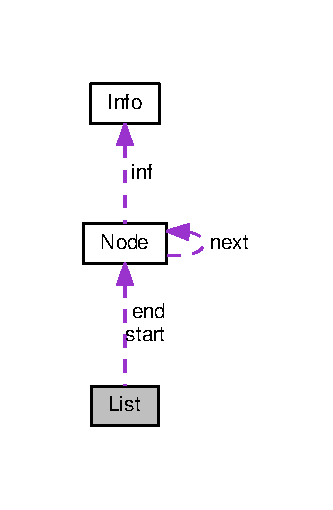
\includegraphics[width=160pt]{struct_list__coll__graph}
\end{center}
\end{figure}
\subsection*{Data Fields}
\begin{DoxyCompactItemize}
\item 
\hypertarget{struct_list_a6a771a8ed404bc96256d21e69e4fc00a}{\hyperlink{link__list_8h_a682f531e759e6edca2fba6c56a0b6298}{node} $\ast$ {\bfseries start}}\label{struct_list_a6a771a8ed404bc96256d21e69e4fc00a}

\item 
\hypertarget{struct_list_abb9fbdc23146cffbf0092baefefdb8b6}{\hyperlink{link__list_8h_a682f531e759e6edca2fba6c56a0b6298}{node} $\ast$ {\bfseries end}}\label{struct_list_abb9fbdc23146cffbf0092baefefdb8b6}

\item 
\hypertarget{struct_list_a439227feff9d7f55384e8780cfc2eb82}{int {\bfseries size}}\label{struct_list_a439227feff9d7f55384e8780cfc2eb82}

\end{DoxyCompactItemize}


\subsection{Detailed Description}
A list storing all the connections. 

The documentation for this struct was generated from the following file\+:\begin{DoxyCompactItemize}
\item 
/home/onestar/\+Documents/\+Inter\+House\+Quiz/main/src/include/\hyperlink{link__list_8h}{link\+\_\+list.\+h}\end{DoxyCompactItemize}

\hypertarget{struct_node}{\section{Node Struct Reference}
\label{struct_node}\index{Node@{Node}}
}


Structure for storing each connection.  




{\ttfamily \#include $<$link\+\_\+list.\+h$>$}



Collaboration diagram for Node\+:\nopagebreak
\begin{figure}[H]
\begin{center}
\leavevmode
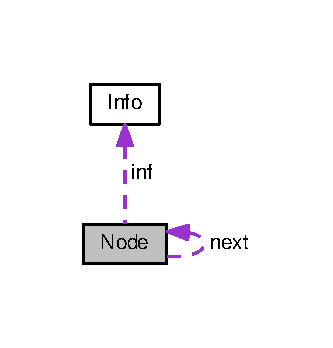
\includegraphics[width=160pt]{struct_node__coll__graph}
\end{center}
\end{figure}
\subsection*{Data Fields}
\begin{DoxyCompactItemize}
\item 
\hypertarget{struct_node_a7a6bf7d3dd8ad7622482a90042e470ef}{struct bufferevent $\ast$ {\bfseries bev}}\label{struct_node_a7a6bf7d3dd8ad7622482a90042e470ef}

\item 
\hypertarget{struct_node_a059d3b39cd7765e831a1a3a5b7195890}{struct \hyperlink{struct_info}{Info} $\ast$ {\bfseries inf}}\label{struct_node_a059d3b39cd7765e831a1a3a5b7195890}

\item 
\hypertarget{struct_node_aa162dd1e0693188a22b1f13b9a2a0ef0}{struct \hyperlink{struct_node}{Node} $\ast$ {\bfseries next}}\label{struct_node_aa162dd1e0693188a22b1f13b9a2a0ef0}

\end{DoxyCompactItemize}


\subsection{Detailed Description}
Structure for storing each connection. 

The documentation for this struct was generated from the following file\+:\begin{DoxyCompactItemize}
\item 
/home/onestar/\+Documents/\+Inter\+House\+Quiz/main/src/include/\hyperlink{link__list_8h}{link\+\_\+list.\+h}\end{DoxyCompactItemize}

\hypertarget{struct_score}{\section{Score Struct Reference}
\label{struct_score}\index{Score@{Score}}
}
\subsection*{Data Fields}
\begin{DoxyCompactItemize}
\item 
\hypertarget{struct_score_aa5fb5a0021da3b9526e4ce8cc490815d}{int {\bfseries score\+\_\+table} \mbox{[}6\mbox{]}}\label{struct_score_aa5fb5a0021da3b9526e4ce8cc490815d}

\item 
\hypertarget{struct_score_ad0901e096b9f3bd4aec771a7cfe5c06a}{char {\bfseries address} \mbox{[}50\mbox{]}}\label{struct_score_ad0901e096b9f3bd4aec771a7cfe5c06a}

\end{DoxyCompactItemize}


The documentation for this struct was generated from the following file\+:\begin{DoxyCompactItemize}
\item 
/home/onestar/\+Documents/\+Inter\+House\+Quiz/main/src/include/score.\+h\end{DoxyCompactItemize}

\hypertarget{struct_u_t__hash__bucket}{\section{U\+T\+\_\+hash\+\_\+bucket Struct Reference}
\label{struct_u_t__hash__bucket}\index{U\+T\+\_\+hash\+\_\+bucket@{U\+T\+\_\+hash\+\_\+bucket}}
}


Collaboration diagram for U\+T\+\_\+hash\+\_\+bucket\+:\nopagebreak
\begin{figure}[H]
\begin{center}
\leavevmode
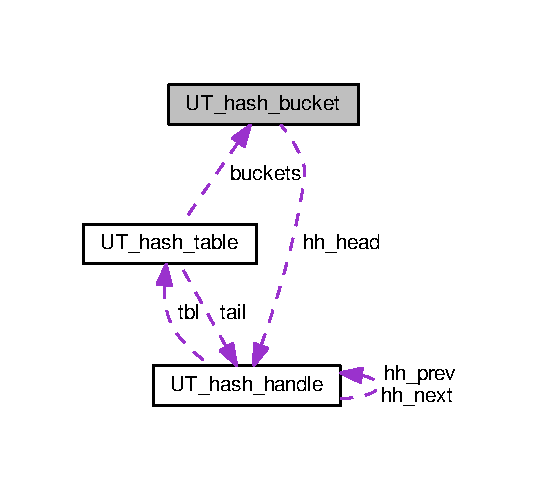
\includegraphics[width=260pt]{struct_u_t__hash__bucket__coll__graph}
\end{center}
\end{figure}
\subsection*{Data Fields}
\begin{DoxyCompactItemize}
\item 
\hypertarget{struct_u_t__hash__bucket_a32d33f384f3c99c1fd80202e1cd64c0c}{struct \hyperlink{struct_u_t__hash__handle}{U\+T\+\_\+hash\+\_\+handle} $\ast$ {\bfseries hh\+\_\+head}}\label{struct_u_t__hash__bucket_a32d33f384f3c99c1fd80202e1cd64c0c}

\item 
\hypertarget{struct_u_t__hash__bucket_a6a9e89d63eb610dfe238b0a840979421}{unsigned {\bfseries count}}\label{struct_u_t__hash__bucket_a6a9e89d63eb610dfe238b0a840979421}

\item 
\hypertarget{struct_u_t__hash__bucket_a49a220a340de3b9ed14648a82472ab84}{unsigned {\bfseries expand\+\_\+mult}}\label{struct_u_t__hash__bucket_a49a220a340de3b9ed14648a82472ab84}

\end{DoxyCompactItemize}


The documentation for this struct was generated from the following file\+:\begin{DoxyCompactItemize}
\item 
/home/onestar/\+Documents/\+Inter\+House\+Quiz/main/src/include/uthash.\+h\end{DoxyCompactItemize}

\hypertarget{struct_u_t__hash__handle}{\section{U\+T\+\_\+hash\+\_\+handle Struct Reference}
\label{struct_u_t__hash__handle}\index{U\+T\+\_\+hash\+\_\+handle@{U\+T\+\_\+hash\+\_\+handle}}
}


Collaboration diagram for U\+T\+\_\+hash\+\_\+handle\+:\nopagebreak
\begin{figure}[H]
\begin{center}
\leavevmode
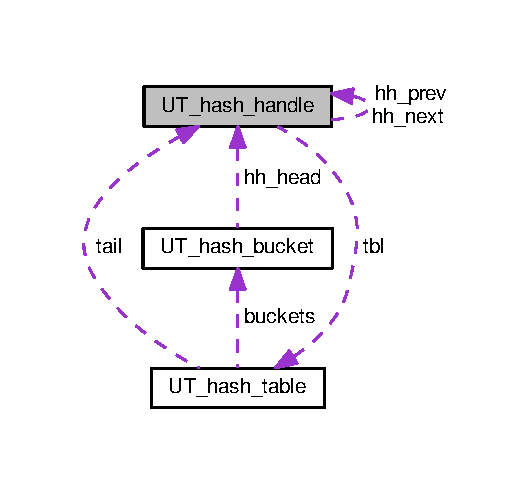
\includegraphics[width=255pt]{struct_u_t__hash__handle__coll__graph}
\end{center}
\end{figure}
\subsection*{Data Fields}
\begin{DoxyCompactItemize}
\item 
\hypertarget{struct_u_t__hash__handle_af0deeb3fe5f35a4c85d105090b498c8d}{struct \hyperlink{struct_u_t__hash__table}{U\+T\+\_\+hash\+\_\+table} $\ast$ {\bfseries tbl}}\label{struct_u_t__hash__handle_af0deeb3fe5f35a4c85d105090b498c8d}

\item 
\hypertarget{struct_u_t__hash__handle_af714e69444763fb9a76ec901a014baf1}{void $\ast$ {\bfseries prev}}\label{struct_u_t__hash__handle_af714e69444763fb9a76ec901a014baf1}

\item 
\hypertarget{struct_u_t__hash__handle_a75b19ffcca77bfc647ff02695958fd95}{void $\ast$ {\bfseries next}}\label{struct_u_t__hash__handle_a75b19ffcca77bfc647ff02695958fd95}

\item 
\hypertarget{struct_u_t__hash__handle_a079301c7093356547fb4601a85503c01}{struct \hyperlink{struct_u_t__hash__handle}{U\+T\+\_\+hash\+\_\+handle} $\ast$ {\bfseries hh\+\_\+prev}}\label{struct_u_t__hash__handle_a079301c7093356547fb4601a85503c01}

\item 
\hypertarget{struct_u_t__hash__handle_a42ef2993dcaaebd656c4a40d174e0c78}{struct \hyperlink{struct_u_t__hash__handle}{U\+T\+\_\+hash\+\_\+handle} $\ast$ {\bfseries hh\+\_\+next}}\label{struct_u_t__hash__handle_a42ef2993dcaaebd656c4a40d174e0c78}

\item 
\hypertarget{struct_u_t__hash__handle_ab5c000aec752f2206131e183daf5efbf}{void $\ast$ {\bfseries key}}\label{struct_u_t__hash__handle_ab5c000aec752f2206131e183daf5efbf}

\item 
\hypertarget{struct_u_t__hash__handle_a4563ea2b1ae1597aa9fd62e005d447b4}{unsigned {\bfseries keylen}}\label{struct_u_t__hash__handle_a4563ea2b1ae1597aa9fd62e005d447b4}

\item 
\hypertarget{struct_u_t__hash__handle_ae73531e09ac884600d96a71ad9afbfa4}{unsigned {\bfseries hashv}}\label{struct_u_t__hash__handle_ae73531e09ac884600d96a71ad9afbfa4}

\end{DoxyCompactItemize}


The documentation for this struct was generated from the following file\+:\begin{DoxyCompactItemize}
\item 
/home/onestar/\+Documents/\+Inter\+House\+Quiz/main/src/include/uthash.\+h\end{DoxyCompactItemize}

\hypertarget{struct_u_t__hash__table}{\section{U\+T\+\_\+hash\+\_\+table Struct Reference}
\label{struct_u_t__hash__table}\index{U\+T\+\_\+hash\+\_\+table@{U\+T\+\_\+hash\+\_\+table}}
}


Collaboration diagram for U\+T\+\_\+hash\+\_\+table\+:\nopagebreak
\begin{figure}[H]
\begin{center}
\leavevmode
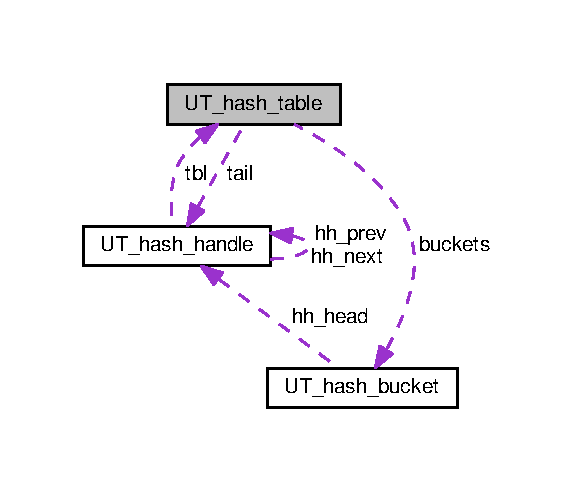
\includegraphics[width=276pt]{struct_u_t__hash__table__coll__graph}
\end{center}
\end{figure}
\subsection*{Data Fields}
\begin{DoxyCompactItemize}
\item 
\hypertarget{struct_u_t__hash__table_ab8166e712e5eff3106991bec13d9ab20}{\hyperlink{struct_u_t__hash__bucket}{U\+T\+\_\+hash\+\_\+bucket} $\ast$ {\bfseries buckets}}\label{struct_u_t__hash__table_ab8166e712e5eff3106991bec13d9ab20}

\item 
\hypertarget{struct_u_t__hash__table_a5f0f25a07827aacb7af4ba2fc4afb5fe}{unsigned {\bfseries num\+\_\+buckets}}\label{struct_u_t__hash__table_a5f0f25a07827aacb7af4ba2fc4afb5fe}

\item 
\hypertarget{struct_u_t__hash__table_a1e4983525460bc9180bbb5e7b404cdbb}{unsigned {\bfseries log2\+\_\+num\+\_\+buckets}}\label{struct_u_t__hash__table_a1e4983525460bc9180bbb5e7b404cdbb}

\item 
\hypertarget{struct_u_t__hash__table_a0f665ec9c648f93c0c529372051e79e7}{unsigned {\bfseries num\+\_\+items}}\label{struct_u_t__hash__table_a0f665ec9c648f93c0c529372051e79e7}

\item 
\hypertarget{struct_u_t__hash__table_af2d4a4fd9335f9813df1ecd3d7124f24}{struct \hyperlink{struct_u_t__hash__handle}{U\+T\+\_\+hash\+\_\+handle} $\ast$ {\bfseries tail}}\label{struct_u_t__hash__table_af2d4a4fd9335f9813df1ecd3d7124f24}

\item 
\hypertarget{struct_u_t__hash__table_af7a888099092eb93f240f1b2bfcc2708}{ptrdiff\+\_\+t {\bfseries hho}}\label{struct_u_t__hash__table_af7a888099092eb93f240f1b2bfcc2708}

\item 
\hypertarget{struct_u_t__hash__table_a0eed5348057e127cdc2fe87bc635a7ac}{unsigned {\bfseries ideal\+\_\+chain\+\_\+maxlen}}\label{struct_u_t__hash__table_a0eed5348057e127cdc2fe87bc635a7ac}

\item 
\hypertarget{struct_u_t__hash__table_a57d93a760aeccec5dad6fac71e9d92ad}{unsigned {\bfseries nonideal\+\_\+items}}\label{struct_u_t__hash__table_a57d93a760aeccec5dad6fac71e9d92ad}

\item 
\hypertarget{struct_u_t__hash__table_ad2dea912f78ea416489b0a386ad0daf9}{unsigned {\bfseries ineff\+\_\+expands}}\label{struct_u_t__hash__table_ad2dea912f78ea416489b0a386ad0daf9}

\item 
\hypertarget{struct_u_t__hash__table_a35073018f3ebb189c76eed44ff19899a}{unsigned {\bfseries noexpand}}\label{struct_u_t__hash__table_a35073018f3ebb189c76eed44ff19899a}

\item 
\hypertarget{struct_u_t__hash__table_acd2a6284879dded65f0b8daa7c68485a}{uint32\+\_\+t {\bfseries signature}}\label{struct_u_t__hash__table_acd2a6284879dded65f0b8daa7c68485a}

\end{DoxyCompactItemize}


The documentation for this struct was generated from the following file\+:\begin{DoxyCompactItemize}
\item 
/home/onestar/\+Documents/\+Inter\+House\+Quiz/main/src/include/uthash.\+h\end{DoxyCompactItemize}

\chapter{File Documentation}
\hypertarget{link__list_8h}{\section{/home/onestar/\+Documents/\+Inter\+House\+Quiz/main/src/include/link\+\_\+list.h File Reference}
\label{link__list_8h}\index{/home/onestar/\+Documents/\+Inter\+House\+Quiz/main/src/include/link\+\_\+list.\+h@{/home/onestar/\+Documents/\+Inter\+House\+Quiz/main/src/include/link\+\_\+list.\+h}}
}


Linked list for storing the current connections.  


\subsection*{Data Structures}
\begin{DoxyCompactItemize}
\item 
struct \hyperlink{struct_node}{Node}
\begin{DoxyCompactList}\small\item\em Structure for storing each connection. \end{DoxyCompactList}\item 
struct \hyperlink{struct_list}{List}
\begin{DoxyCompactList}\small\item\em A list storing all the connections. \end{DoxyCompactList}\end{DoxyCompactItemize}
\subsection*{Typedefs}
\begin{DoxyCompactItemize}
\item 
\hypertarget{link__list_8h_a682f531e759e6edca2fba6c56a0b6298}{typedef struct \hyperlink{struct_node}{Node} \hyperlink{link__list_8h_a682f531e759e6edca2fba6c56a0b6298}{node}}\label{link__list_8h_a682f531e759e6edca2fba6c56a0b6298}

\begin{DoxyCompactList}\small\item\em Structure for storing each connection. \end{DoxyCompactList}\item 
\hypertarget{link__list_8h_a109860c2e14bbeb03ea3d54a112ce4f2}{typedef struct \hyperlink{struct_list}{List} \hyperlink{link__list_8h_a109860c2e14bbeb03ea3d54a112ce4f2}{list}}\label{link__list_8h_a109860c2e14bbeb03ea3d54a112ce4f2}

\begin{DoxyCompactList}\small\item\em A list storing all the connections. \end{DoxyCompactList}\end{DoxyCompactItemize}
\subsection*{Functions}
\begin{DoxyCompactItemize}
\item 
\hyperlink{link__list_8h_a682f531e759e6edca2fba6c56a0b6298}{node} $\ast$ \hyperlink{link__list_8h_a00b335e95c7a5d601ceb46a7195abafb}{list\+Search} (const struct bufferevent $\ast$bev, const \hyperlink{link__list_8h_a109860c2e14bbeb03ea3d54a112ce4f2}{list} $\ast$the\+List)
\begin{DoxyCompactList}\small\item\em Searching the connection using the address. and port. \end{DoxyCompactList}\item 
void \hyperlink{link__list_8h_a658cc3d2128a7207a96f75b2837e4c55}{list\+Create} (struct \hyperlink{struct_list}{List} $\ast$$\ast$\hyperlink{link__list_8h_a109860c2e14bbeb03ea3d54a112ce4f2}{list})
\begin{DoxyCompactList}\small\item\em Create and initialize the linked list. \end{DoxyCompactList}\item 
void \hyperlink{link__list_8h_aa1ec9c8b9f1c56f861e653508a4a832f}{list\+Add} (struct bufferevent $\ast$bev, struct \hyperlink{struct_info}{Info} $\ast$\hyperlink{structinfo}{info}, struct \hyperlink{struct_list}{List} $\ast$\hyperlink{link__list_8h_a109860c2e14bbeb03ea3d54a112ce4f2}{list})
\begin{DoxyCompactList}\small\item\em Create and add a new node into the list. \end{DoxyCompactList}\item 
void \hyperlink{link__list_8h_a87c5c319d01ed2a866d9e42d116da21b}{list\+Remove} (struct \hyperlink{struct_node}{Node} $\ast$\hyperlink{link__list_8h_a682f531e759e6edca2fba6c56a0b6298}{node}, struct \hyperlink{struct_list}{List} $\ast$\hyperlink{link__list_8h_a109860c2e14bbeb03ea3d54a112ce4f2}{list})
\begin{DoxyCompactList}\small\item\em Remove the node from the list. \end{DoxyCompactList}\item 
void \hyperlink{link__list_8h_a6da5203fd20a34d1d9d9a07fdf339e0f}{list\+Print} (struct \hyperlink{struct_list}{List} $\ast$\hyperlink{link__list_8h_a109860c2e14bbeb03ea3d54a112ce4f2}{list})
\begin{DoxyCompactList}\small\item\em Print the node to wprintw(). \end{DoxyCompactList}\item 
void \hyperlink{link__list_8h_ab8a7cdec2167d1f1de1c732d06528154}{list\+Delete} (struct \hyperlink{struct_list}{List} $\ast$\hyperlink{link__list_8h_a109860c2e14bbeb03ea3d54a112ce4f2}{list})
\begin{DoxyCompactList}\small\item\em Delete all the nodes in the list. \end{DoxyCompactList}\item 
int \hyperlink{link__list_8h_a66a143a1ccdc887eba693b933a347d3c}{list\+Broadcast} (\hyperlink{link__list_8h_a109860c2e14bbeb03ea3d54a112ce4f2}{list} $\ast$, char $\ast$)
\begin{DoxyCompactList}\small\item\em Broadcast the msg to all connections in the list. \end{DoxyCompactList}\end{DoxyCompactItemize}
\subsection*{Variables}
\begin{DoxyCompactItemize}
\item 
\hypertarget{link__list_8h_a4c82b9b311bc880c5cf25a6a07fe1925}{struct \hyperlink{struct_list}{List} $\ast$ {\bfseries the\+List}}\label{link__list_8h_a4c82b9b311bc880c5cf25a6a07fe1925}

\end{DoxyCompactItemize}


\subsection{Detailed Description}
Linked list for storing the current connections. 

\begin{DoxyAuthor}{Author}
Steven Chien 

Star Poon (\href{mailto:oneonestar@gmail.com}{\tt oneonestar@gmail.\+com}) 
\end{DoxyAuthor}
\begin{DoxyVersion}{Version}
1.\+0 
\end{DoxyVersion}
\begin{DoxyDate}{Date}
2013-\/2014 
\end{DoxyDate}
\begin{DoxyCopyright}{Copyright}
G\+N\+U General Public License v3.\+0 
\end{DoxyCopyright}


\subsection{Function Documentation}
\hypertarget{link__list_8h_aa1ec9c8b9f1c56f861e653508a4a832f}{\index{link\+\_\+list.\+h@{link\+\_\+list.\+h}!list\+Add@{list\+Add}}
\index{list\+Add@{list\+Add}!link\+\_\+list.\+h@{link\+\_\+list.\+h}}
\subsubsection[{list\+Add}]{\setlength{\rightskip}{0pt plus 5cm}void list\+Add (
\begin{DoxyParamCaption}
\item[{struct bufferevent $\ast$}]{bev, }
\item[{struct {\bf Info} $\ast$}]{info, }
\item[{struct {\bf List} $\ast$}]{list}
\end{DoxyParamCaption}
)}}\label{link__list_8h_aa1ec9c8b9f1c56f861e653508a4a832f}


Create and add a new node into the list. 


\begin{DoxyParams}{Parameters}
{\em bev} & the bufferevent bounded to that connection. \\
\hline
{\em info} & the info structure bounded to that connection. \\
\hline
{\em list} & the bufferevent send to the callback function. \\
\hline
\end{DoxyParams}
\hypertarget{link__list_8h_a66a143a1ccdc887eba693b933a347d3c}{\index{link\+\_\+list.\+h@{link\+\_\+list.\+h}!list\+Broadcast@{list\+Broadcast}}
\index{list\+Broadcast@{list\+Broadcast}!link\+\_\+list.\+h@{link\+\_\+list.\+h}}
\subsubsection[{list\+Broadcast}]{\setlength{\rightskip}{0pt plus 5cm}int list\+Broadcast (
\begin{DoxyParamCaption}
\item[{{\bf list} $\ast$}]{, }
\item[{char $\ast$}]{}
\end{DoxyParamCaption}
)}}\label{link__list_8h_a66a143a1ccdc887eba693b933a347d3c}


Broadcast the msg to all connections in the list. 


\begin{DoxyParams}{Parameters}
{\em list} & the \hyperlink{struct_list}{List} structure which containing the connections. \\
\hline
{\em msg} & the message wanted to broadcast. \\
\hline
\end{DoxyParams}
\hypertarget{link__list_8h_a658cc3d2128a7207a96f75b2837e4c55}{\index{link\+\_\+list.\+h@{link\+\_\+list.\+h}!list\+Create@{list\+Create}}
\index{list\+Create@{list\+Create}!link\+\_\+list.\+h@{link\+\_\+list.\+h}}
\subsubsection[{list\+Create}]{\setlength{\rightskip}{0pt plus 5cm}void list\+Create (
\begin{DoxyParamCaption}
\item[{struct {\bf List} $\ast$$\ast$}]{list}
\end{DoxyParamCaption}
)}}\label{link__list_8h_a658cc3d2128a7207a96f75b2837e4c55}


Create and initialize the linked list. 


\begin{DoxyParams}{Parameters}
{\em list} & the bufferevent send to the callback function. \\
\hline
\end{DoxyParams}
\hypertarget{link__list_8h_ab8a7cdec2167d1f1de1c732d06528154}{\index{link\+\_\+list.\+h@{link\+\_\+list.\+h}!list\+Delete@{list\+Delete}}
\index{list\+Delete@{list\+Delete}!link\+\_\+list.\+h@{link\+\_\+list.\+h}}
\subsubsection[{list\+Delete}]{\setlength{\rightskip}{0pt plus 5cm}void list\+Delete (
\begin{DoxyParamCaption}
\item[{struct {\bf List} $\ast$}]{list}
\end{DoxyParamCaption}
)}}\label{link__list_8h_ab8a7cdec2167d1f1de1c732d06528154}


Delete all the nodes in the list. 


\begin{DoxyParams}{Parameters}
{\em list} & The \hyperlink{struct_list}{List} structure which containing the connections. \\
\hline
\end{DoxyParams}
\hypertarget{link__list_8h_a6da5203fd20a34d1d9d9a07fdf339e0f}{\index{link\+\_\+list.\+h@{link\+\_\+list.\+h}!list\+Print@{list\+Print}}
\index{list\+Print@{list\+Print}!link\+\_\+list.\+h@{link\+\_\+list.\+h}}
\subsubsection[{list\+Print}]{\setlength{\rightskip}{0pt plus 5cm}void list\+Print (
\begin{DoxyParamCaption}
\item[{struct {\bf List} $\ast$}]{list}
\end{DoxyParamCaption}
)}}\label{link__list_8h_a6da5203fd20a34d1d9d9a07fdf339e0f}


Print the node to wprintw(). 


\begin{DoxyParams}{Parameters}
{\em list} & The \hyperlink{struct_list}{List} structure which containing the connections. \\
\hline
\end{DoxyParams}
\hypertarget{link__list_8h_a87c5c319d01ed2a866d9e42d116da21b}{\index{link\+\_\+list.\+h@{link\+\_\+list.\+h}!list\+Remove@{list\+Remove}}
\index{list\+Remove@{list\+Remove}!link\+\_\+list.\+h@{link\+\_\+list.\+h}}
\subsubsection[{list\+Remove}]{\setlength{\rightskip}{0pt plus 5cm}void list\+Remove (
\begin{DoxyParamCaption}
\item[{struct {\bf Node} $\ast$}]{node, }
\item[{struct {\bf List} $\ast$}]{list}
\end{DoxyParamCaption}
)}}\label{link__list_8h_a87c5c319d01ed2a866d9e42d116da21b}


Remove the node from the list. 


\begin{DoxyParams}{Parameters}
{\em node} & The node needed to be removed from the list. \\
\hline
{\em list} & The \hyperlink{struct_list}{List} structure which containing the connections. \\
\hline
\end{DoxyParams}
\hypertarget{link__list_8h_a00b335e95c7a5d601ceb46a7195abafb}{\index{link\+\_\+list.\+h@{link\+\_\+list.\+h}!list\+Search@{list\+Search}}
\index{list\+Search@{list\+Search}!link\+\_\+list.\+h@{link\+\_\+list.\+h}}
\subsubsection[{list\+Search}]{\setlength{\rightskip}{0pt plus 5cm}{\bf node}$\ast$ list\+Search (
\begin{DoxyParamCaption}
\item[{const struct bufferevent $\ast$}]{bev, }
\item[{const {\bf list} $\ast$}]{the\+List}
\end{DoxyParamCaption}
)}}\label{link__list_8h_a00b335e95c7a5d601ceb46a7195abafb}


Searching the connection using the address. and port. 


\begin{DoxyParams}{Parameters}
{\em bev} & the bufferevent send to the callback function. \\
\hline
{\em the\+List} & the linked list containin the connections. \\
\hline
\end{DoxyParams}

\begin{DoxyRetVals}{Return values}
{\em return} & null if not found. \\
\hline
\end{DoxyRetVals}

%--- End generated contents ---

% Index
\newpage
\phantomsection
\addcontentsline{toc}{chapter}{Index}
\printindex

\end{document}
